\documentclass[final,paperwidth=36in,paperheight=48in,portrait,fontscale=0.3]{baposter}
% NIPS Workshops format

% Encoding.
\usepackage[utf8]{inputenc}
\usepackage[T1]{fontenc}

\usepackage{graphicx} % Required for including images
\usepackage{subfig}
\usepackage{booktabs} % for professional tables
\usepackage{floatrow}
\usepackage{float}

\usepackage{textgreek}
\usepackage{pstricks}
\usepackage{tikz}
\usepackage{pgf}
\usepackage{placeins} % For \FloatBarrier
\usetikzlibrary{positioning}
\usepackage{environ}
\makeatletter
\newsavebox{\measure@tikzpicture}
\NewEnviron{scaletikzpicturetowidth}[1]{%
	\def\tikz@width{#1}%
	\def\tikzscale{1}\begin{lrbox}{\measure@tikzpicture}%
		\BODY
	\end{lrbox}%
	\pgfmathparse{#1/\wd\measure@tikzpicture}%
	\edef\tikzscale{\pgfmathresult}%
	\BODY
}
\makeatother

\usepackage{amsmath} % For typesetting math
\usepackage{amssymb} % Adds new symbols to be used in math mode

\usepackage{booktabs} % Top and bottom rules for tables
\usepackage{enumitem} % Used to reduce itemize/enumerate spacing
%\usepackage{palatino} % Use the Palatino font
\renewcommand{\familydefault}{\sfdefault}
\usepackage[font=small,labelfont=bf]{caption} % Required for specifying captions to tables and figures

\usepackage{multicol} % Required for multiple columns
\setlength{\columnsep}{1.5em} % Slightly increase the space between columns
\setlength{\columnseprule}{0mm} % No horizontal rule between columns
\usepackage{multirow}


\newcommand{\compresslist}{ % Define a command to reduce spacing within itemize/enumerate environments, this is used right after \begin{itemize} or \begin{enumerate}
\setlength{\itemsep}{1pt}
\setlength{\parskip}{0pt}
\setlength{\parsep}{0pt}
}

% Defines the color used for content box headers
\definecolor{lightblue}{cmyk}{0.83,0.24,0,0.16}
%\definecolor{lightblue}{rgb}{0.145,0.6666,1}

%%%%%%%%%%%%%%%%%%%%%%%%%%%%%%%%%%%%%%%%%%%%%%%%%%%%%%%%%%%%%%%%%%%%%%%%%%%%%%
%%% Begin of Document
%%%%%%%%%%%%%%%%%%%%%%%%%%%%%%%%%%%%%%%%%%%%%%%%%%%%%%%%%%%%%%%%%%%%%%%%%%%%%%

% Pojedyncze spacje po kropce.
\frenchspacing

\begin{document}



\hyphenation{resolution occlusions}
%%
\begin{poster}%
  % Poster Options
  {
  % Show grid to help with alignment
  grid=false,
  % Column spacing
  colspacing=1em,
  % Color style
  bgColorOne=white,
  bgColorTwo=white,
  borderColor=lightblue,
  headerColorOne=black,
  headerColorTwo=lightblue,
  headerFontColor=white,
  boxColorOne=white,
  boxColorTwo=lightblue,
  % Format of textbox
  textborder=roundedleft,
%  textborder=faded,
  % Format of text header
  eyecatcher=true,
  headerborder=closed,
  columns=2,
  headerheight=4cm,
%  textfont=\sc, An example of changing the text font
  headershape=roundedright,
  headershade=shadelr,
  headerfont=\Large\bf\textsc, %Sans Serif
  textfont={\setlength{\parindent}{1.5em}\large},
  boxshade=plain,
%  background=shade-tb,
  background=plain,
  linewidth=1pt
  } 
  { % Left Eye Catcher - IBM logo

\includegraphics[width=4cm]{../img/ibm_research.png}
  } 
  % Title
  	{\bf\textsc{On transfer learning using a MAC model variant}\vspace{0.2em}}
  % Authors
  {
	\textbf{Vincent Marois, T.S. Jayram, Vincent Albouy, Tomasz Kornuta, \\Younes Bouhadjar, Ahmet S. Ozcan}\\

	\texttt{\{vmarois,jayram,tkornut,byounes,asozcan\}@us.ibm.com},{\{vincent.albouy\}@ibm.com}\\
  }
  { % Left Eye Catcher

\includegraphics[width=4cm]{../img/arc_logo.png}
  }


% A coloured circle useful as a bullet with an adjustably strong filling
\newcommand{\colouredcircle}{%
\tikz{\useasboundingbox (-0.2em,-0.32em) rectangle(0.2em,0.32em); \draw[draw=black,fill=lightblue,line width=0.03em] (0,0) circle(0.16em);}}
\tikzstyle{block} = [draw,minimum size=2.5em, outer sep=2]

%%%%%%%%%%%%%%%%%%%%%%%%%%%%%%%%%%%%%%%%%%%%%%%%%%%%%%%%%%%%%%%%%%%%%%%%%%%%%%%

\headerbox{Abstract}{name=abstract,column=0,row=0}{
We introduce a variant of the MAC model (Hudson and Manning, ICLR 2018) with a simplified set of equations that achieves comparable accuracy, while training faster. We evaluate both models on CLEVR and CoGenT, and show that, transfer learning with fine-tuning results in a 15 point increase in accuracy, matching the state of the art. Finally, in contrast, we demonstrate that improper fine-tuning can actually reduce a model's accuracy as well.
} %headerbox

\headerbox{The MAC Model}{name=double-pendulum, column=0, below=abstract}{
	\begin{figure}[H]
		\centering
		\subfloat[]{{
				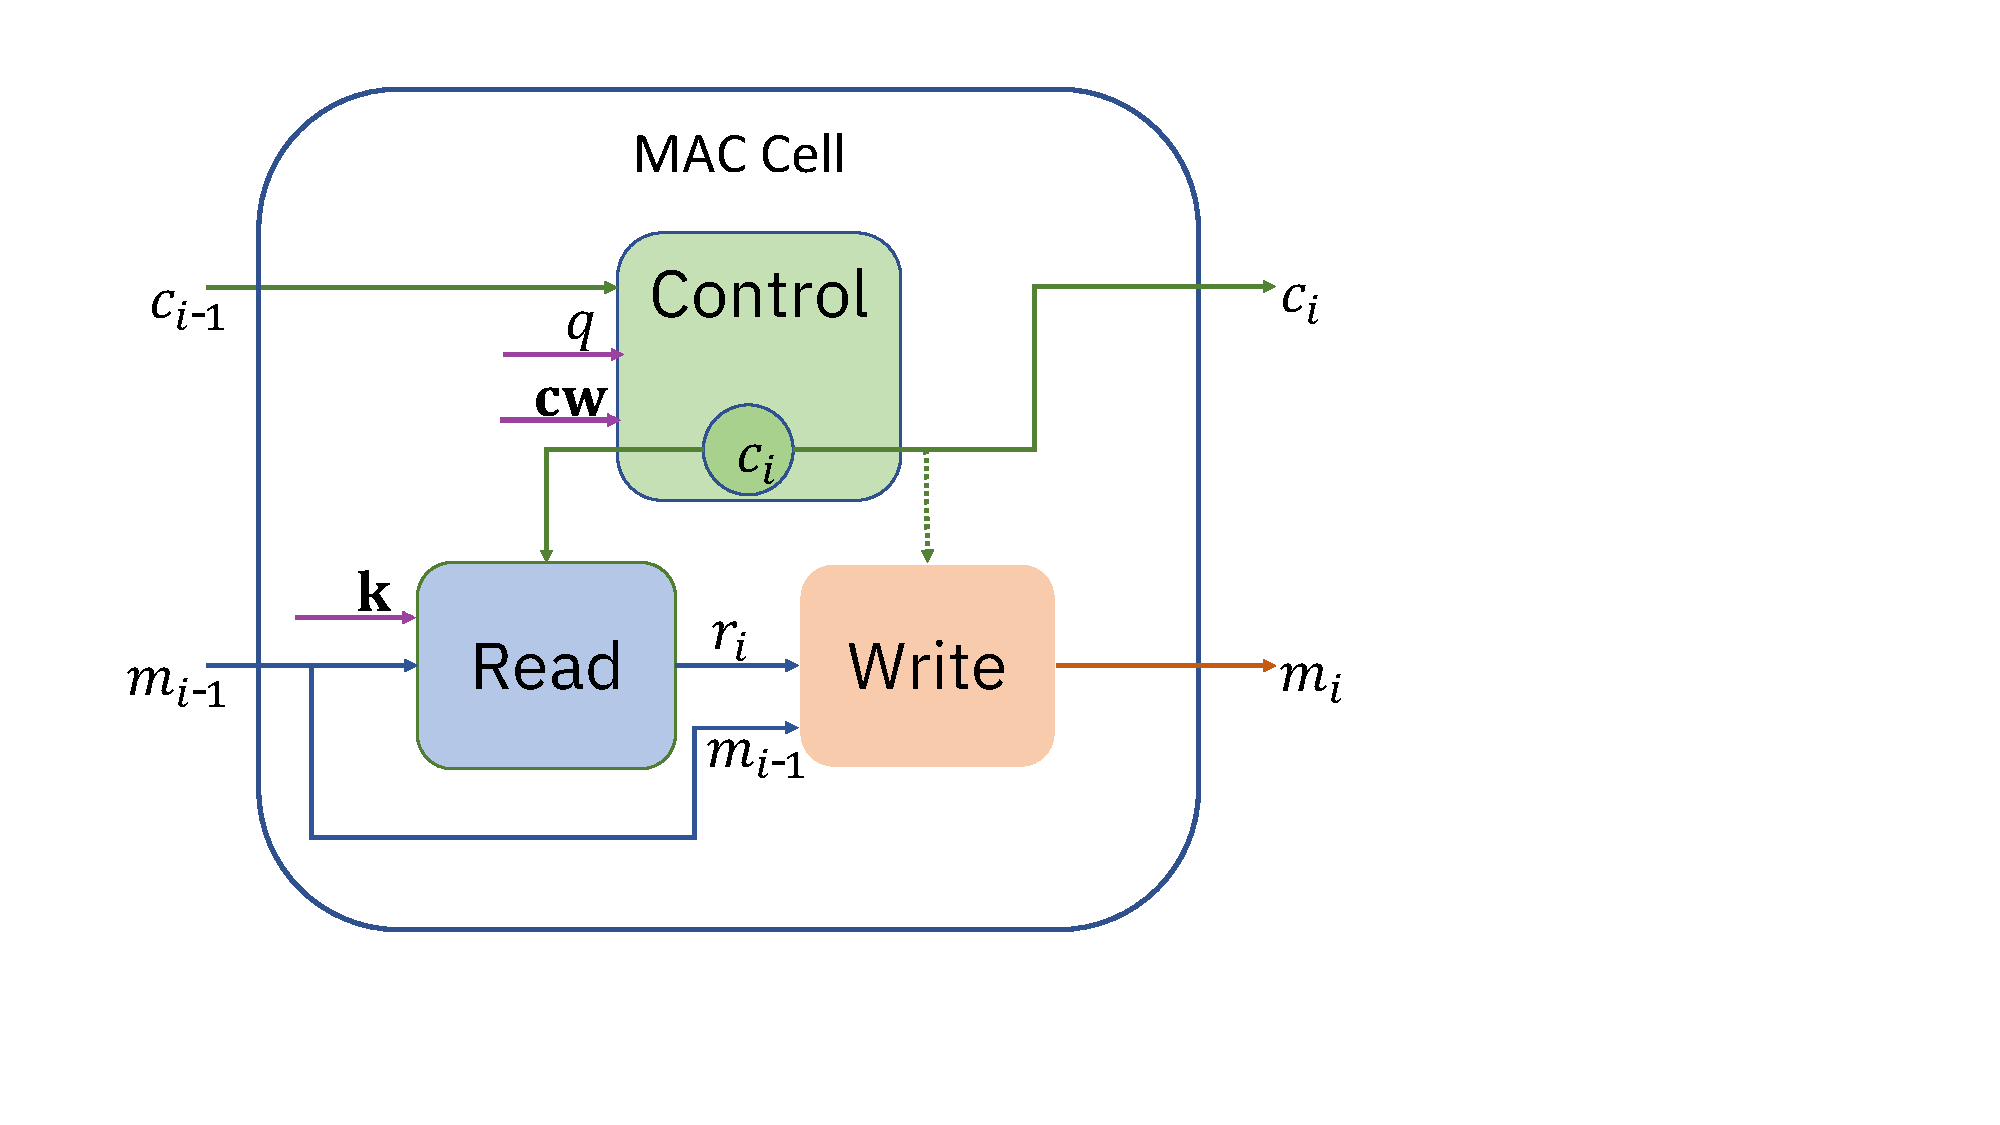
\includegraphics[width=0.60\textwidth]{../img/mac_cell.pdf}
				\label{subfig:pendulum_picture}
		}}
	
		\caption{The MAC cell}
		\label{fig:pendulum}
	\end{figure}
	
The MAC network is a recurrent model that performs sequential reasoning,  where each step involves analyzing a part of the question followed by shifting the attention over the image. The core of the model is the MAC cell, supported with an input unit that processes the question and image pair, and output unit which produces the answer.  The input unit uses an LSTM to process the question in a word-by-word manner producing a sequence of contextual words and a final question representation. Besides, the input unit utilizes a pre-trained ResNet followed by two CNN layers to extract a feature map (referred to as knowledge base) from the image.
}

\headerbox{Simplified Mac Model}{name=data acquisition, column=0, below=double-pendulum}{

}

\headerbox{Transfer Learning - Experiments}{name=dataset, column=1}{
}

\headerbox{MAC failures examples on CLEVR}{name=baseline, column=1, below=dataset}{
	{
	}

		{

	}
}

\headerbox{References}{name=references, column=1, below=baseline}{
	\small
	\vspace{-8pt}
	\renewcommand{\refname}{}
	\bibliographystyle{abbrv}
	\bibliography{sample}
	\normalsize
	\textsl{}
	\begin{center}
		The Double Pendulum Chaotic Dataset:
		\large
		\texttt{\color{blue} https://ibm.github.io/double-pendulum-chaotic-dataset/}
	\end{center}
}

\end{poster}

\end{document}